\section{Theorie}
\label{sec:Theorie}

\subsection{Grundlagen zu Mikrowellen und Hohlleitern}
\label{subsec:grundlagen}
Mikrowellen sind elektromagnetische Wellen im Frequenzbereich von \SI{300}{\mega\Hz}
bis \SI{300}{\giga\Hz}. Daher sind sie sehr gut für Hohlleiter geeignet, da diese in einem
Frequenzbereich von \SI{1}{\giga\Hz} bis \SI{200}{\giga\Hz} arbeiten. Ein Hohlleiter ist
ein Metallrohr, durch das elektromagnetische Wellen verlustarm geleitet werden können.
Sehr gängig sind dabei Rechteckhohlleiter, auf die auch im Folgenden weiter eingegangen
werden soll.

Jeder Hohlleiter kann verschiedene Formen von Wellen, auch Moden genannt, leiten.
Die Moden unterscheiden sich in der Verteilung des elektrischen und des magnetischen
Feldes. Man unterscheidet TE-Moden, bei denen das elektrische Feld transversal zur
Ausbreitungsrichtung der Welle und TM-Moden, bei denen das magnetische Feld transversal
zur Ausbreitungsrichtung schwingt. Ein spezialfall sind TEM-Moden, bei denen sowohl
das elektrische, als auch das magnetische Feld transversal zur Ausbreitungsrichtung
schwingt. Für jede Mode im Hohlleiter existiert eine untere Grenzfrequenz, unterhalb
der kein Energietransport im Hohlleiter möglich ist. Sie kommt durch die Abmessungen
des Hohlleiters und die damit verbundenen Randbedingungen bei der Lösung der Wellengleichung zustande.

Im freien Raum gilt der Zusammenhang
\begin{equation}
  c= \lambda_0 f\,.
  \label{eqn:frequenz}
\end{equation}
Dabei ist $c$ die Lichtgeschwindigkeit im Vakuum, $\lambda_0$ die Wellenlänge im
freien Raum und $f$ die Frequenz der Welle.
Für TE- und TM-Moden in einem lufgefüllten Hohlleiter gilt
\begin{align}
  \lambda_{\symup{g}}&=\frac{\lambda_0}{\sqrt{1-\left(\frac{\lambda_0}
  {\lambda_{\symup{c}}}\right)^2}} \,, \label{eqn:hohlleiterg}\\
  \lambda_{\symup{c}}&=\frac{2}{\sqrt{\left(\frac{m}{a}\right)^2+
  \left(\frac{n}{b}\right)^2}} \,.
  \label{eqn:hohlleiterc}
\end{align}
Hier ist $\lambda_{\symup{g}}$ die Wellenlänge im Hohlleiter und $\lambda_{\symup{c}}$
die Grenzwellenlänge im Hohlleiter. Die Abmessungen $a$ und $b$ beschreiben Länge und Breite des Hohlleiters.
Die Moden werden durch Angabe der Zahlen $m$ und $n$ genauer bestimmt.
Wie an diesen Formeln zu erkennen ist, ist die Wellenlänge im Hohlleiter
größer als die der selben Wellen im freien Raum.

%Wird im Hohhleiter ein Teil der Welle an einer Störstelle reflektiert, so bildet
%sich eine stehende Welle.
Wird im Hohlleiter ein Teil der Welle an einer Störstelle reflektiert, so interferieren
einfallende und reflektierte Welle. Aufgrund der hohen Frequenz der Mikrowelle kann praktisch nur eine
Einhüllende gemessen werden, bei der sich Minima und Maxima ausbilden,
%Es bilden sich also Minima und Maxima der Einhüllenden
%aus,
wobei zwei Minima bzw. zwei Maxima eine halbe Wellenlänge voneinander entfernt
sind. Für diese Wellen kann ein Stehwellenverhältnis oder auch SWR (Standing Wave
Ratio) berechnet werden. Für dieses gilt
\begin{equation}
  S=\frac{E_{\symup{max}}}{E_{\symup{min}}}=\frac{|E_{\symup{ein}}|+|E_{\symup{refl}}|}
  {|E_{\symup{ein}}|-|E_{\symup{refl}}|}\,.
\end{equation}
In Abbildung \ref{fig:swr} ist das Stehwellenverähltnis visualisiert.
\begin{figure}
  \centering
  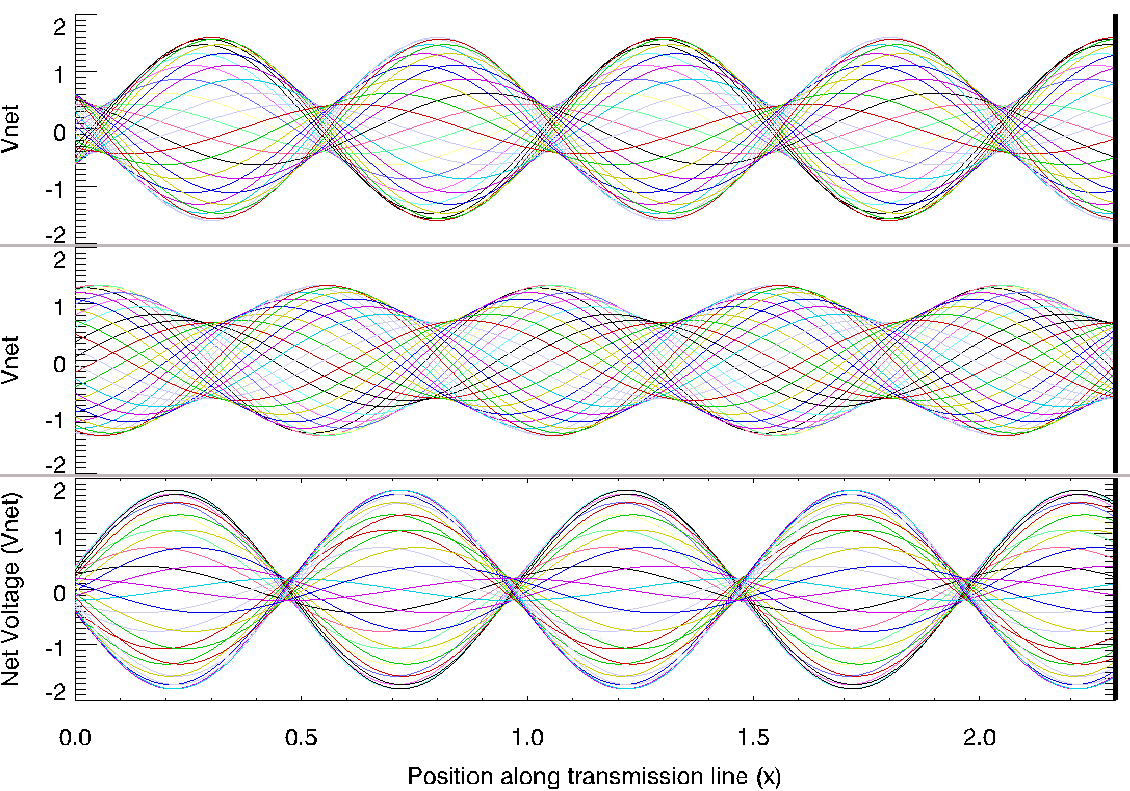
\includegraphics[width=\textwidth]{data/swr.png}
  \caption{Visualisierung des Stehwellenverhältnisses. Gezeigt sind SWR von 4, 2 und 9 \cite{wiki}.}
  \label{fig:swr}
\end{figure}



\subsection{Das Reflexklystron}
\label{subsec:klystron}
Mikrowellen können durch verschiedene Bauteile erzeugt werden. Ein besonders häufig
verwendetes Bauteil ist das Reflexklystron. Eine Skizze zur Funktionsweise desselben
befindet sich in Abbildung \ref{fig:klystron}.

\begin{figure}
  \centering
  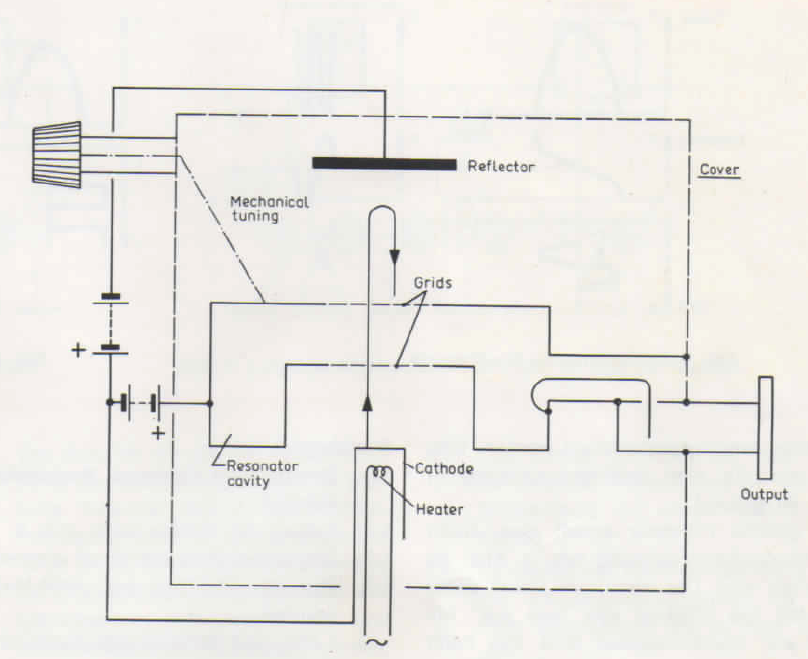
\includegraphics[width=300pt]{data/klystron.png}
  \caption{Skizze zur Funktionsweise eines Klystrons \cite{Versuchsanleitung_alt}.}
  \label{fig:klystron}
\end{figure}

Es besteht im Wesentlichen aus einem torusförmigen Hohlraum, der als LC Resonanzkreis
dient. Im Betrieb schwingt dieser Kreis, was auch zu einer Schwingung des elektrischen
und magnetischen Feldes im Inneren führt. Im Hohlraum ist eine Kopplungsschleife
angebracht, die durch elektromagnetische Induktion das Signal auskoppeln kann.

Da ein LC Kreis aufgrund des Widerstandes nicht ewig weiterschwingen kann und ihm
zusätzlich Leistung entzogen wird, bedarf es einer Methode, um ihm Energie zuzuführen.
Dafür treten aus einer Glühwendel Elektronen aus, die daraufhin zu einer Kathode hin
beschleunigt werden. Danach durchlaufen sie das elektrische Feld zwischen den beiden
Gittern. Dabei können sie, je nach Phase der Schwingung, auf ein beschleunigendes
oder auf ein abbremsendes elektrisches Feld stoßen. Nach dem Durchgang durch die Gitter fliegen sie in das entgegengesetzt
zur Kathode ausgerichtete Reflektorfeld, in dem sie in die andere Richtung beschleunigt
werden. Daraufhin kehren die Elektronen zum Gitter zurück, wo sie erneut entweder
abgebremst oder beschleunigt werden. Diejenigen Elektronen, die abgebremst werden,
deponieren dabei Energie im elektrischen Feld des Resonators. Somit kann der LC Kreis
in Schwingung gehalten werden.

Die größten Resonanzeffekte treten gerade dann auf, wenn die Verweildauer der Elektron im Resonater
gleich ($3/4 + n$), mit $n$ als einer natürlichen Zahl (inklusive Null), mal der Periodendauer des Schwingkreises ist. Das Ziel ist es, diesen Modus zu erreichen, um
eine maximale Leistung zu generieren.\\
Eine Modulation der Frequenz und der Amplitude der Mikrowellen ist sowohl durch eine mechanische Abstimmung, also zum Beispiel eine Änderung des Hohlraumresonatorvolumens, als auch durch elektronische Abstimmung möglich. Dies umfasst das Anlegen unterschiedlicher Wechselspannungen als Reflektorspannungen.
